%%
%% Copyright 2007-2020 Elsevier Ltd
%%
%% This file is part of the 'Elsarticle Bundle'.
%% ---------------------------------------------
%%
%% It may be distributed under the conditions of the LaTeX Project Public
%% License, either version 1.2 of this license or (at your option) any
%% later version.  The latest version of this license is in
%%    http://www.latex-project.org/lppl.txt
%% and version 1.2 or later is part of all distributions of LaTeX
%% version 1999/12/01 or later.
%%
%% The list of all files belonging to the 'Elsarticle Bundle' is
%% given in the file `manifest.txt'.
%%

%% Template article for Elsevier's document class `elsarticle'
%% with numbered style bibliographic references
%% SP 2008/03/01
%%
%%
%%
%% $Id: elsarticle-template-num.tex 190 2020-11-23 11:12:32Z rishi $
%%
%%
\documentclass[preprint,12pt]{elsarticle}

%% Use the option review to obtain double line spacing
%% \documentclass[authoryear,preprint,review,12pt]{elsarticle}

%% Use the options 1p,twocolumn; 3p; 3p,twocolumn; 5p; or 5p,twocolumn
%% for a journal layout:
%% \documentclass[final,1p,times]{elsarticle}
%% \documentclass[final,1p,times,twocolumn]{elsarticle}
%% \documentclass[final,3p,times]{elsarticle}
%% \documentclass[final,3p,times,twocolumn]{elsarticle}
%% \documentclass[final,5p,times]{elsarticle}
%% \documentclass[final,5p,times,twocolumn]{elsarticle}

%% For including figures, graphicx.sty has been loaded in
%% elsarticle.cls. If you prefer to use the old commands
%% please give \usepackage{epsfig}

%% The amssymb package provides various useful mathematical symbols
\usepackage{amssymb}
%% The amsthm package provides extended theorem environments
%% \usepackage{amsthm}
\usepackage{graphicx}
%\usepackage{caption}
\usepackage{comment}
\usepackage{amsmath}
\usepackage{subfigure}
\usepackage{booktabs}
\usepackage{float}
%\usepackage{pgfplots}
\usepackage{graphicx}
\usepackage{fullpage} % for full page width
\usepackage{lipsum} % for dummy text
\usepackage{adjustbox} % for adjusting graphics

\usepackage{hyperref}
\hypersetup{
     colorlinks=true,
     linkcolor=black,
     citecolor=black,
     filecolor=black,
     urlcolor=black,
 }

%% The lineno packages adds line numbers. Start line numbering with
%% \begin{linenumbers}, end it with \end{linenumbers}. Or switch it on
%% for the whole article with \linenumbers.
%% \usepackage{lineno}

\journal{Computer Methods in Applied Mechanics and Engineering}

\begin{document}

\begin{frontmatter}

%% Title, authors and addresses

%% use the tnoteref command within \title for footnotes;
%% use the tnotetext command for theassociated footnote;
%% use the fnref command within \author or \address for footnotes;
%% use the fntext command for theassociated footnote;
%% use the corref command within \author for corresponding author footnotes;
%% use the cortext command for theassociated footnote;
%% use the ead command for the email address,
%% and the form \ead[url] for the home page:
%% \title{Title\tnoteref{label1}}
%% \tnotetext[label1]{}
%% \author{Name\corref{cor1}\fnref{label2}}
%% \ead{email address}
%% \ead[url]{home page}
%% \fntext[label2]{}
%% \cortext[cor1]{}
%% \affiliation{organization={},
%%             addressline={},
%%             city={},
%%             postcode={},
%%             state={},
%%             country={}}
%% \fntext[label3]{}

\title{Enhancing Fractographic Fatigue Failure Analysis, Automated Flow Stress, and Fracture Toughness Evaluation in Fatigue Specimens - a Smart Approach with Artificial Intelligence and Image Processing}

%% use optional labels to link authors explicitly to addresses:
%% \author[label1,label2]{}
%% \affiliation[label1]{organization={},
%%             addressline={},
%%             city={},
%%             postcode={},
%%             state={},
%%             country={}}
%%
%% \affiliation[label2]{organization={},
%%             addressline={},
%%             city={},
%%             postcode={},
%%             state={},
%%             country={}}
\author[Computer_b]{Or Anijar}
\author[Computer_a]{Jonatan Boritski}
\author[Computer_a]{Sapir Dahan}
\author[soreq]{Elad Farkash}
\author[Computer_a]{Avichay Mazin}
\author[technion]{Shmuel Osovski}
\author[fracture]{Mor Mega}
%\author[Computer_a,Computer_a,Computer_b]{Avichay Mazin$^a$, Jonatan Boritski$^a$, Or Anijar$^b$, Sapir Dahan$^a$, Elad Farkash$^c$, Mor Mega$^d$}

\affiliation[Computer_a]{organization={Department of Computer Science, \\Ariel University},%Department and Organization
            city={Ariel},
            postcode={40700},
            country={Israel}}

\affiliation[Computer_b]{organization={Department of Computer Science, \\Ariel University},%Department and Organization
            city={Ariel},
            postcode={40700},
            country={Israel}}

\affiliation[soreq]{organization={Soreq Nuclear Research Center},%Department and Organization
            city={Yavne},
            postcode={81800},
            country={Israel}}

\affiliation[fracture]{organization={The Fracture and Fatigue Research Laboratory, \\Department of Mechanical Engineering and Mechatronics, \\Ariel University},%Department and Organization
            city={Ariel},
            postcode={40700},
            country={Israel}}

\affiliation[technion]{organization={Faculty of Mechanical Engineering, Technion - Israel Institute of Technology},%Department and Organization
city={Haifa},
postcode={32000},
country={Israel}}

\begin{abstract}
%% Text of abstract

\end{abstract}

%%Graphical abstract
\begin{graphicalabstract}
%\includegraphics{grabs}
\end{graphicalabstract}

%%Research highlights
\begin{highlights}
\item Research highlight 1
\item Research highlight 2
\end{highlights}

\begin{keyword}
%% keywords here, in the form: keyword \sep keyword

%% PACS codes here, in the form: \PACS code \sep code

%% MSC codes here, in the form: \MSC code \sep code
%% or \MSC[2008] code \sep code (2000 is the default)

\end{keyword}

\end{frontmatter}

%% \linenumbers

%% main text
\section{Introduction}
\label{Sec:Introduction}

\begin{comment}
\subsection{Today Scene: What We Have and What Might Evolve}  \label{Subsec:Today's Scene: What We Have and What Might Evolve}
The application of machine learning and deep learning for analyzing fracture surfaces and extracting meaningful information has seen a significant rise in the last years as discussed in a study \cite{tsopanidis2020unsupervised}.
As we can see in the article, these tools are not only facilitate the extraction of valuable insights that may surpass the capabilities of traditional fractographic experts, but also introduce automation, making the entire process more efficient and time saving.

In practical terms, utilizing machine and deep learning for fracture surface analysis proves to be a time saving effort. Instead of the manual analysis of fracture surfaces, which can be time consuming, these advanced tools simplify the process. Moreover, the accuracy and effectiveness of the analyses are often hig enough that, in certain cases, reliance on traditional fractographic experts may become unnecessary. The automated nature of machine and deep learning analyses contributes to a more efficient, rapid, and sometimes even superior understanding of fracture surfaces.
\par
As we explain earlier, an analysis of fatigue failure in engineering structures has already been done before in some aspects.
For example, in previous studies, some researchers have already made an analysis about fractions materials produced through 3D printing. One is the research \cite{anidjar2023transfer}.
 This research emphasize why is important to analyze fractures in materials and explain that fractographic analysis plays a crucial role in understanding the mechanical properties and fatigue behavior of materials, especially in identifying the primary causes of failure. For this problem, the challenge of identifying fatigue crack initiation sites, the researchers attitude towards the solution for the problem was innovation and efficiency. They recognized that the process of identifying and characterizing fatigue crack initiation sites in materials can be time consuming and costly when done manually. Therefore, they try to develop a computer vision based approach that could automate and expedite the process.
the researchers have been used in two deep learning algorithms. One is called ResNet152 and it used to filter out image sections that do not contain the fatigue crack initiation site. The second is called YOLOv5 which used for object detection. After the irrelevant image sections have been filtered out by ResNet152, YOLOv5 is trained to detect and classify the remaining image sections to precisely identify the initiation site.
\end{comment}


%\subsection{Mechanical Background}
Additive Manufacturing (AM) technology, also known as 3D printing, is an innovative process wherein parts are fabricated layer by layer, adhering to three-dimensional digital models. This innovative technique, emerged in the late 1980s, has made a significant advancement in manufacturing technology. Widely referred as a cornerstone of the third industrial revolution, AM offers almost unlimited opportunities for the creation of intricately designed products, which is markedly different from traditional metal manufacturing methods~\cite{wong2012review}. One of the big advantage of AM lies in its obviation of the need for molds, a factor that substantially diminishes production costs and enable producing of complex components~\cite{herzog2016additive}.


Titanium alloys are highly advanced structural materials known for their diverse set of exceptional properties. These include resistance to corrosion in seawater, impressive strength-to-weight ratios, excellent fracture toughness, high fatigue resistance, strong compatibility with composites, long-term durability with minimal maintenance requirements, and exceptional biocompatibility~\cite{qian2016additive}. Despite the extensive exploration of the static mechanical properties of AM materials, encompassing factors such as strength, stiffness, and impact energy~\cite{debroy2018additive,gorsse2017additive}, investigations into their dynamic performance and fatigue characteristics remain comparatively scant. Additive Ti-6Al-4V is increasingly esteemed as promising lightweight structural components in aerospace and automotive sectors~\cite{boyer1996overview,debroy2018additive}. In these areas, the ability to withstand fatigue loads is critical. However, a comprehensive understanding of its fatigue behavior and underlying failure mechanisms remains elusive. Hence, delving into the mechanical fatigue properties of AM materials becomes imperative.

Fatigue failure of engineering components and structures results from progressive fracture caused by cyclic or fluctuating loads. Fatigue is an important potential cause of mechanical failure because most engineering components or structures can be subjected to cyclic loads during their lifetime.
An abbreviated summary of fatigue processes and mechanisms: fatigue crack initiation, propagation, and final fracture. Characteristic fatigue fracture features that can be visually discerned under low magnification are then described.
Typical microscopic features observed on structural metals are presented.
\begin{comment}
    In \textcolor{red}{need more up to date papers if these are examples for papers that made use of the method we are using... If not, then examples of what are these?}~\cite{astiz1986incompatible,carpinteri1992stress,carpinteri1992elliptical}, models for predicting the stress intensity factor for such a geometry were proposed.
\end{comment}
\textcolor{green}{Additive Manufacturing\\Fatigue\\Fractografic analysis and surface regions\\stress intensity factor calculation models\\flow stress calculation models\\It may be useful to solve this using computer vision methods  (no equations, just references)}




%\subsection{Related Work}  \label{Subsec:Related Work}
    The integration of computer vision in the field of fracture mechanics, particularly in the analysis of metal fractures, has evolved significantly over recent years.
    In its early stages, the approach primarily relied on scanning Scanning Electron Microscope (SEM) images and conducting manual classification efforts.
    However, the traditional process is manual, labor-intensive, and prone to human error.
    Automating this process and developing quantitative methods for studying fracture surfaces is a major challenge but has significant industrial and scientific potential.
    Automated fractography could enhance the reliability of failure analysis and uncover new insights into material failure mechanisms.

    Early applications in fracture mechanics prioritized image processing over the more advanced computer vision and machine learning techniques.
    These initial approaches were designed to enhance features in images of fracture surfaces captured by SEM and optical microscopy, with a greater emphasis on qualitative rather than quantitative analysis.
    Fundamental techniques employed in these efforts included spatial domain methods like texture analysis and the Gray Level Co-occurrence Matrix (GLCM) for fractal analysis.
    \textcolor{red}{In \cite{zain2009enhancement}}, the authors experimented with various spatial filtering techniques such as mean, median, Gaussian, and Wiener filters to enhance the quality of identification of the fracture image.
    In the engineering field, another set of experiments can be observed \textcolor{red}{In \cite{das2011characterization}}, where the changes on the surface are effectively characterized using these methods.
    Furthermore, some of these techniques also incorporated transform domain methods, such as Fourier transform, wavelet transform, and Gabor transform.
    In another study, \textcolor{red}{In \cite{hu2017automation}}, the authors employed edge detection and peak-finding algorithms to determine the progression marks associated with fatigue crack growth.

    These methods were applied to optical and Scanning Electron Microscopy (SEM) images to classify and characterize fracture surfaces.
    However, these methods often required additional user input and assumptions, which limited their robustness and applicability, especially for complex surfaces.

    Recent developments have seen the use of machine learning and artificial intelligence in materials characterization, including micro-structure classification and defect analysis.
    Promising machine learning methods like artificial neural networks and support vector machines have played a pivotal role in classifying observed fractures, yielding promising results in materials characterization.
    Some notable achievements in this area include the use of a complex CNN architecture known as Unet,
    as demonstrated \textcolor{red}{In \cite{tsopanidis2020toward}}, where an accuracy of 71.2 percent in Intersection over Union (IOU) was achieved for triple-class classification,
    distinguishing inter-granular and trans-granular fracture events from scanning electron microscope images.
    Another article compared a more intricate Unet neural network architecture, reaching an accuracy of 0.86 percent in the Dice score accuracy metric for the segmentation task of detecting dimple fractures.

    A prominent trend has emerged in recent times where a fusion of traditional image processing methods and cutting-edge AI techniques has been observed.
    In these approaches, a pivotal role is played by feature extraction during the prepossessing phase, enhancing the salient characteristics within images.
    As exemplified \textcolor{red}{In \cite{naik2019identification}}, researchers combined texture recognition algorithms, specifically the Local Binary Pattern (LBP), with the classical machine algorithm called Linear Discriminant Analysis (LDA). This innovative combination allowed them to identify the fracture type and its area in both brittle and ductile materials by leveraging the uniqueness of texture features, achieving an impressive accuracy rate of 94 percent.
    Another notable example is presented \textcolor{red}{In \cite{bastidas2016fractographic}}, where SVM classification was employed.

    A groundbreaking advancement in this research lies in the integration of the localization problem with the feature extraction phase.
    As demonstrated \textcolor{red}{In \cite{zhang2023automated}}, a remarkable achievement was reached with a detection rate of up to 92 percent in terms of the F1 score for detecting bridge cracks.
    This approach was developed by segmenting the process into three distinct phases: initially selecting specific regions, then extracting features using methods like SIFT and HOG, and finally applying the YOLO neural network architecture for precise object localization and detection.


\textcolor{green}{In this study,...}






\section{Mechanical basic terms}  \label{sec:Basic terms}


Two failure criteria may be used to predict the final failure of a specimen subjected to cyclic fatigue loading. The first criterion is related to the flow stress parameter \(\sigma_{net}\), and the second is related to the stress intensity factor \(K_{I}\). Once one of these parameters reaches a critical value, failure is expected. The model used here to determine the flow stress in a bar specimen tested in cyclic fatigue is presented in Section~\ref{Subsec: Flow stress calculation model}.
In Section~\ref{Subsec: Stress intensity factors calculation model}, several closed-form solutions for the determination of \(K_I\) are introduced and the best one is chosen \cite{shin2004experimental}.


\subsection{Fractographic image analysis description}
\label{Subsec: Fractographic image analysis}

\subsection{Flow stress calculation model}
\label{Subsec: Flow stress calculation model}
\begin{figure*}[t!]
  \begin{center}
  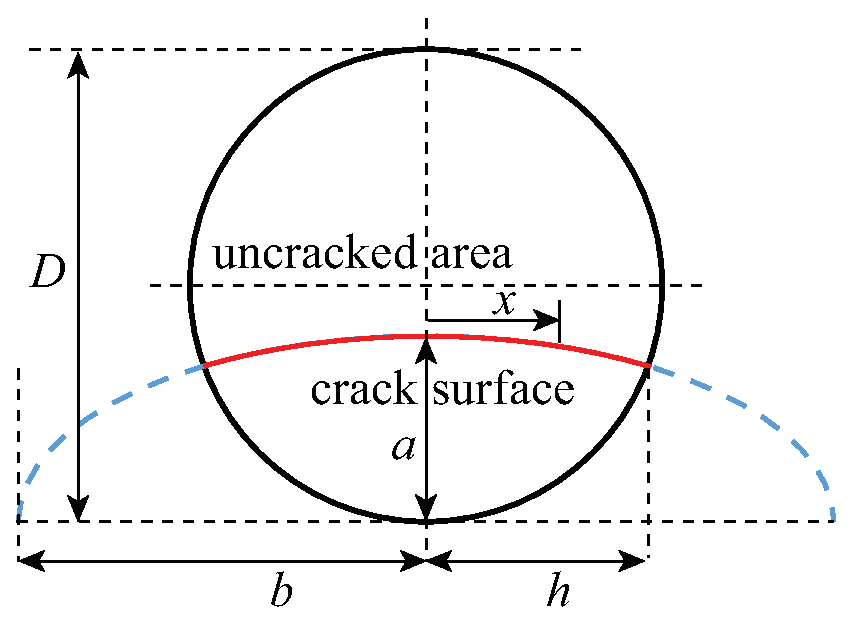
\includegraphics[width=3in]{elliptical_surface_crack.eps}
  \caption{Schematic view of an elliptical crack.}
  \label{fig:elliptical_crack}
   \end{center}
\end{figure*}

One known failure criterion is based on the calculated flow stress $\sigma_{net}$. Once this parameter reaches the failure stress $\sigma_{f}$, the final failure will occur.

The failure stress \(\sigma_{f}\) is related to the ligament area, defined as the uncracked area illustrated in Fig.~\ref{fig:elliptical_crack}. For a specific material, the value of \(\sigma_{f}\) is given by \cite{kanchanomai2004low}
%
\begin{equation}
    \sigma_{f} = \frac{\sigma_Y + \sigma_{UTS}}{2}
\end{equation}
%
where \(\sigma_Y\) is the yield stress and \(\sigma_{UTS}\) is the ultimate stress of the material.

The flow stress, \(\sigma_{net}\), is a function of the applied force and the uncracked area, namely,
%
\begin{equation}
\label{eq:sig_net}
\sigma_{net}= \displaystyle\frac{\sigma_{max} A_0}{A_{\textit{uncracked area}}}
\end{equation}
%
where $\sigma_{max}$ is the maximum applied stress in each fatigue cycle, \(A_0\) is the total area of the specimen surface, and \(A_{\text{uncracked area}}\) is the ligament area illustrated in Fig.~\ref{fig:elliptical_crack}. Once \(\sigma_{net}\) reaches the value of \(\sigma_f\), the specimen will fail.
%
%

\subsection{Stress intensity factor calculation model}
\label{Subsec: Stress intensity factors calculation model}
\textcolor{green}{add ellipse restrictions}
%
%
\begin{table}[t!]
\caption{Tabulated values of $M_{i,j,k}$ in eq.~(\ref{eq:F_I}). \strut}
\label{tab:M_ijk}      % Give a unique label
\resizebox{\columnwidth}{!}{
\begin{tabular}{cccclccclccc}
\noalign{\bigskip}\hline\noalign{\smallskip}\hline
  &          & k=0       &           &  &          & k=1       &          &  &         & k=2      &           \\ \cline{2-4} \cline{6-8} \cline{10-12}
j & i=0      & 1         & 2         &  & i=0      & 1         & 2        &  & i=0     & 1        & 2         \\
0 & 1.095    & -1.177    & 0.725     &  & 0.113    & 0.271     & -0.388   &  & -0.896  & 0.904    & 0.008     \\
1 & -1.336   & 17.924    & -17.427   &  & 1.824    & -11.649   & 10.074   &  & 3.092   & 0.701    & -4.883    \\
2 & 13.108   & -137.252  & 134.652   &  & -21.709  & 98.358    & -80.088  &  & -4.197  & -32.641  & 55.092    \\
3 & -43.689  & 545.816   & -551.902  &  & 105.483  & -415.027  & 328.165  &  & -13.255 & 204.104  & -305.079  \\
4 & 134.868  & -1223.334 & 1239.493  &  & -271.225 & 982.713   & -772.921 &  & 51.548  & -568.407 & 916.962   \\
5 & -242.653 & 1541.587  & -1548.537 &  & 387.47   & -1329.634 & 1055.952 &  & -59.329 & 857.543  & -1545.428 \\
6 & 254.093  & -1006.656 & 969.388   &  & -290.024 & 961.893   & -784.581 &  & 13.481  & -657.659 & 1372.595  \\
7 & -108.196 & 264.206   & -227.132  &  & 88.387   & -288.565  & 245.798  &  & 10.854  & 191.57   & -485.556  \\
\hline\noalign{\smallskip}\hline
\end{tabular}
}
\end{table}
An additional known failure criterion is based on the stress intensity factor $K_I$ value. Once this parameter reaches the fracture toughness $K_{Ic}$ of the tested material, the crack will propagate, and final failure will occur. The critical stress intensity factor or fracture toughness value \(K_{Ic}\) is reached once the crack approaches a critical size.



In~\cite{toribio2009automated}, it was demonstrated that the crack front in a fatigue bar specimen may be treated as an ellipse with the center located at the specimen surface, as illustrated in Fig.~\ref{fig:elliptical_crack}. The parameters $a$ and $b$ are the major and minor diameters of the ellipse in Fig.~\ref{fig:elliptical_crack}, respectively. These dimensions represent the depth and width of the crack, respectively. The parameter $D$ is the total specimen diameter, $x$ is a chosen coordinate between 0 and $h$ where $h$ is the horizontal distance between the center of the ellipse and the intersection between the ellipse and the specimen outer surface. It may be noted that the axis of symmetry of the ellipse is the same as the axis of symmetry of the bar and the center of the ellipse is on the edge of the rod. All parameters are shown in Fig.~\ref{fig:elliptical_crack} and may be used to calculate $K_I$.

Next, several closed-form solution are presented and the best one is chosen. In~\cite{valiente1980criterios}, the first closed-form solution was introduced. This form was only for a straight front crack ($b$ limit to infinity). The value of $K_I$ is calculated only at the center of the crack front.
In~\cite{astiz1986incompatible}, a closed-form solution is introduced for an elliptical crack front; but $K_I$ is found only in the center of the crack front. In~\cite{couroneau1998simplified,carpinteri1992elliptical} two closed-form solution were presented, one at the crack front center, shown as point A in Fig.~\ref{fig:elliptical_crack}, and another for the end of the crack front, shown as point G in Fig.~\ref{fig:elliptical_crack}. In \cite{shin2004experimental} a closed-form solution was found based on the FE method and the virtual crack extension technique~\cite{hellen1975method}. The solution was found as a function of $a$, $b$ and $x/h$ the location along the crack front, as shown in Fig.~\ref{fig:elliptical_crack}.
Another solution that use these three parameters~\cite{shih2002stress} was found to produce negative results. A detailed review on these solutions and other solutions may be found in~\cite{toribio2009automated}.
It was found~\cite{toribio2009automated} that the best closed-form solution for the problem in this research is~\cite{shih2002stress}.



\begin{comment}
The three dimensionless parameters used are the crack depth $H$, the ellipse ratio $r$, and the location along the crack front $X$. These parameters may be calculated as
\begin{equation}\label{eq:crack depth}
    H=\frac{D}{a}\;\;\;;\;\;\; r=\frac{a}{b} \;\;\;;\;\;\;X=\frac{x}{h}
\end{equation}
where $D$ and $a$ are the specimen diameter and the largest distance between the specimen surface and the ellipse along the specimen diameter, $a$ and $b$ are the major and minor diameters of the ellipse, $x$ is a chosen parameter between 0 and $h$ and $h$ is the horizontal distance between the center of the ellipse and the intersection between the ellipse and the specimen outer surface. All illustrated are illustrated in Fig.~(\ref{}).
\end{comment}



In~\cite{shin2004experimental}, the closed-form solution is based on the FE method and the virtual crack extension technique~\cite{hellen1975method}.  The calculation of \(K_I\) is proposed as
%
\begin{equation}
\label{eq:K_I__F_I}
K_{I}=F_I \sigma_0 \sqrt{\pi a}
\end{equation}
%
where $F_I$ is a function of $a, b, D, h$ and $x$ given as
%
\begin{equation}
\label{eq:F_I}
F_{I}=\sum^{2}_{i=0} \sum^{7}_{j=0}\sum^{2}_{k=0} M_{ijk}\left(\frac{a}{b}\right)^i  \left(\frac{a}{D}\right)^j  \left(\frac{x}{h}\right)^k\;\;.
\end{equation}
In eq.~(\ref{eq:F_I}) the coefficients $M_{ijk}$ were determined from FEAs in \cite{shin2004experimental} and presented in Table~\ref{tab:M_ijk}.







\section{Neural network terms}
A neural network is a computational model inspired by the human brain's neural connections, composed of interconnected nodes organized into layers. It excels at learning patterns from data and can perform tasks such as image recognition, image segmentation, language processing, and predictive analytics. What makes neural networks special is their ability to autonomously discern intricate patterns and relationships, allowing them to adapt and make accurate predictions or classifications in various domains, making them a cornerstone in artificial intelligence. \\
In the context of image analysis, a specialized neural network architecture known as UNet plays a pivotal role. UNet is particularly acclaimed for its efficacy in image segmentation, where it excels at delineating and categorizing specific features within an image. This segmentation capability is invaluable in applications like medical image analysis and object recognition, providing a nuanced understanding of visual data.\\
Moreover, the incorporation of heatmaps improves the interpretability of neural network results by providing a visual depiction of the intensity or concentration of recognized features. This is particularly valuable for tasks like pinpointing objects within an image and detecting anomalies. The combined strengths of foundational learning, segmentation proficiency from UNet, and interpretive insights offered by heatmaps collectively propel the capabilities of artificial intelligence across varied and intricate domains.

The U-Net architecture represents a significant advancement in neural networks for image segmentation tasks.
It is structured into two main components: a contracting path on the left side and an expansive path on the right.
The contracting path mirrors a conventional convolutional network structure, featuring convolutional layers followed by rectified linear units (ReLUs) and max pooling operations.
In contrast, the expansive path involves upsampling the feature map and merging it with the corresponding feature map from the contracting path, enhancing information flow through the network.

Image segmentation is the process of dividing an image into distinct regions, is vital for identifying objects and boundaries.
This involves assigning labels to each pixel so that pixels with the same label exhibit similar attributes, such as color, texture, or intensity.
The outcome of this process is either a collection of segments covering the entire image or a set of contours derived from it.

Evaluating the accuracy of image segmentation is crucial, often done by comparing the segmented result against a known 'ground truth'.
Commonly used metrics include the Dice coefficient and the Intersection over Union (IoU),
also known as the Jaccard index.
Both these metrics are formulated as ratios that evaluate the extent of overlap between the predicted segmentation and the ground truth relative to their combined area.

The Dice coefficient is given as $2|X \cap Y|/(|X|+|Y|)$, where $X$ and $Y$ are the predicted segmentation and the ground truth, respectively.
The IoU is given as $|X \cap Y|/|X \cup Y|$.

Both these metrics are pivotal in quantifying the performance of segmentation models, with higher values indicating a greater degree of accuracy in the segmentation task.

Calculating the magnitude of gradients over an image is a preprocessing method designed to enhance the image for easier analysis.
This magnitude indicates the intensity of the gradient at each pixel.
In the study of crack growth, approaching the crack's center usually corresponds to an increase in its magnitude.
The magnitude is computed using the formula
\begin{equation}
\label{eq:magnitude}
M=\sqrt{G_x^2+G_y^2}
\end{equation}
where $G_x$ and $G_y$ are the gradients in the $x$ and $y$ directions, respectively.

It can be achieved by two methods:
\begin{enumerate}
  \item Using the Sobel operator.
  \item Using the Canny edge detector.
\end{enumerate}

The Sobel operator is a discrete differentiation operator, computing an approximation of the gradient of the image intensity function.
At each point in the image, the result of the Sobel operator is either the corresponding gradient vector or the norm of this vector.
The Sobel operator is based on convolving the image with a small, separable, and integer-valued filter in the horizontal and vertical directions and is therefore relatively inexpensive in terms of computations.

The Canny edge detector is an edge detection operator that uses a multi-stage algorithm to detect a wide range of edges in images.

In order two smooth the the gradient, an sliding window is used.
The window is a square of size $n \times n$.
The gradient in each pixel is calculated by the following formula:
\begin{equation}
\label{eq:gradient}
G=\sqrt{\frac{1}{n^2}\sum_{i=1}^{n}\sum_{j=1}^{n}I_{i,j}^2}
\end{equation}
where $I_{i,j}$ is the intensity of the pixel in the $i$ row and $j$ column.



\section{Dataset} \label{Sec:dataset}

The dataset in the research comprises 63 SEM images of Ti-6Al-4V alloy fatigue specimens, captured at a resolution of 4576 by 4096 pixels. Each image provides a detailed view of 5.5 mm with an approximate pixel size of 1.34 $\mu$m, allowing for an in-depth analysis of the specimens microstructures and fracture patterns. The images are categorized based on the print quality recommended by the manufacturer into three groups: 30 images in P1 for standard printing, 21 in P2 for enhanced quality, and 12 in P3 indicating lower quality. Extensive documentation on specimen production and the experimental setup is available in previous work \cite{navickaite2022efficient}, offering a comprehensive context for the SEM images used in this research.

\begin{figure}[h!]
  \centering
  \includegraphics[width=0.8\textwidth]{figures/side_by_side.png}
  \caption{SEM images of a Ti-6Al-4V fatigue specimen from two opposing viewpoints (A and B), showcasing the fracture surfaces from different perspectives.}
  \label{same_material_from_both_sides}
\end{figure}

An important aspect of the dataset is the inclusion of some duplicated images, captured from opposite viewpoints of certain specimens. This feature is crucial for a comprehensive analysis but does not apply to every image in the dataset. The duplicated views ensure that material behavior and fracture details are more thoroughly captured, aiding in the holistic examination of specimen conditions. Figure~\ref{same_material_from_both_sides} provides an example of this, showcasing SEM images of a Ti-6Al-4V fatigue specimen from two opposing viewpoints (A and B), and highlighting the fracture surfaces from different perspectives.





\vspace{\baselineskip}
To tailor the dataset for algorithmic analysis, unnecessary metadata detailing technical specifications such as the view field, working distance (WD), and beam intensity (BI) was removed from each image. This cleansing process was accomplished by cropping the images to a uniform resolution of 4096 by 4096 pixels, thereby eliminating any extraneous data. The primary objective of this preprocessing step was to refine the dataset to ensure that the learning algorithms are focused solely on the pertinent features of the specimens. By concentrating on these relevant aspects, the approach significantly enhances the potential for accurate analysis by the subsequent models. This step, crucial for maintaining the integrity and relevance of the dataset, is depicted in Figure~\ref{steps_was_done} as step '(a)'.


\begin{figure*}[h!]
  \centering
  \includegraphics[width=1\linewidth, height=0.47\textheight]{figures/steps_dataset3.png}
  \caption{Overview of the dataset preparation process: (a) Cropping images to remove metadata and standardize resolution; (b) Division to train and test set, 50 images for training and 13 for test; (c) Reduce resolution to 128*128 pixels for make the UNet models less complicated; (d) Final images with masks applied for model training.}
  \label{steps_was_done}
\end{figure*}


In addition to preprocessing, the dataset underwent augmentation to enhance the robustness of the UNet models without increasing the overall number of images. Augmentation techniques such as rotation, flipping, and scaling were applied to simulate a variety of viewing angles and specimen orientations. This process was essential for preparing the models to recognize and analyze specimens under diverse conditions, thereby improving their ability to generalize from the training data to new, unseen images. Although the dataset size remained unchanged, the augmentation significantly diversified the range of features that the models were exposed to during training.
\vspace{\baselineskip}

Our research utilizes two distinct UNet models designed for complementary analytical tasks. The first model's objective is to extract the external contours of the specimens, effectively separating the subject of interest from the background. The second model focuses on identifying and segmenting regions within the specimens where cracks are present, providing critical insights into areas indicative of material failure.



The manual labeling process was an essential step in preparing the dataset for the training of these models. Experts meticulously annotated the external boundaries of the specimens for contour extraction and marked the regions exhibiting cracks for focused analysis by the second model. This manual intervention ensures that the models are trained on accurate and relevant features, significantly enhancing their analytical capabilities. An example of the labeling process for the two UNet models is shown in Figure~\ref{lables}, where 'A','B','C' are the original image after crop, the external boundary of the specimen that was done manually, and the mask the first UNet will get later as labeld data, accordingly.
'D','E','F' are the original image after crop, the boundary of specimen crack, and the mask the second UNet will get as labeld data, accordingly.

\begin{figure}[h!]
  \centering
  \includegraphics[width=1\textwidth]{figures/lables.png}
  \caption{Manual labeling process illustrated for the two UNet models. The top row ('A', 'B', 'C') demonstrates the stages for external contour detection: 'A' shows the cropped input image, 'B' depicts the manually identified external contour of the specimen, and 'C' presents the generated mask, which serves as labeled data for training the first UNet model. The bottom row ('D', 'E', 'F') outlines the crack detection process: 'D' is the cropped input image, 'E' highlights the manually delineated crack within the specimen, and 'F' shows the corresponding mask created for use as labeled data in training the second UNet model.}
  \label{lables}
\end{figure}

Following this detailed annotation work, the dataset was divided, with 50 images allocated to the training set and the remaining 13 to the test set. This division ensures a robust training regime and an effective evaluation framework for both UNet models, facilitating comprehensive learning and accurate performance assessment.

This division of the dataset into the training and test sets is detailed in Table~\ref{tab:dataset_division}, providing a clear overview of the distribution of images and ensuring a balanced approach for model training and validation.

\begin{table}[htbp]
\centering
\small
\caption{Division of the dataset into training and test sets}
\label{tab:dataset_division}
\begin{tabular}{@{}lcc@{}}
\toprule
\textbf{Dataset} & \textbf{Number of Images} & \textbf{Percentage (\%)} \\ \midrule
Training Set & 50 & 79.37 \\
Test Set & 13 & 20.63 \\ \bottomrule
\textbf{Total} & \textbf{63} & \textbf{100} \\ \bottomrule
\end{tabular}
\end{table}

Through this comprehensive dataset preparation, encompassing precise image selection, preprocessing, manual labeling, and strategic division, we have established a solid foundation for the UNet models. This foundation is critical for accurately analyzing and learning from the SEM images of Ti-6Al-4V fatigue specimens, enhancing the reliability and efficacy of our material failure analysis.


\vspace{\baselineskip}
\vspace{\baselineskip}
\vspace{\baselineskip}




\section{Proposed Artificial Intelligence-driven framework}
\label{Sec: Proposed Artificial intelligence-driven framework}
\subsection{Preliminary Operations}
\label{sec:prelimnary_operations}

In the progression from raw data to a format amenable for deep learning analysis, we employed TensorFlow, an open-source machine learning framework that offers extensive libraries for developing and training AI models. TensorFlow's functionalities were instrumental in our Preliminary Operations, enhancing the dataset readiness for analysis through our dual UNet models and ensuring the data accurately captures the complexities of material fractures.

\subsubsection{Dataset Refinement for Deep Learning}
As part of the dataset refinement, we utilized TensorFlow to resize the images to a manageable resolution of 128x128 pixels. This adjustment balances the necessity of maintaining essential microstructural details against the constraints of computational efficiency. Alongside resizing, TensorFlow facilitated the normalization of each pixel value to a range between 0 and 1. This normalization process standardizes the input data, aiding the models' learning algorithms by providing a consistent scale for image intensities.

\subsubsection{Data Augmentation Strategy}
To bolster the training dataset diversity and better simulate varied imaging conditions, we leveraged TensorFlow data augmentation capabilities. Implementing strategic transformations—rotations, flips, and zooms—augmented the dataset comprehensiveness without distorting the inherent properties of the material microstructures. These steps, crucial for enhancing model robustness and generalizability, underscore TensorFlow pivotal role in preparing data that empowers our models to more accurately identify and classify fracture patterns.

\subsubsection{Model-Specific Adjustments}
Precise adjustments were made to cater to the specialized requirements of our two UNet models. Contrary to the image resizing and normalization tasks where TensorFlow capabilities were leveraged for efficiency, the process of labeling for model training was conducted manually. This manual labeling was crucial for ensuring the accuracy of the dataset, particularly for the tasks at hand. For the model tasked with extracting external contours, establishing a clear demarcation between the specimen and its background was paramount, necessitating a nuanced understanding and interpretation of the images that automated processes could not achieve. Similarly, the manual identification and labeling of internal features such as cracks were critical for the second model, which focuses on internal contour detection. These painstakingly detailed manual annotations ensure that the models receive data that is optimally aligned with their analytical objectives, underscoring the indispensable role of expert knowledge in the initial stages of model preparation. While TensorFlow played a pivotal role in the data preprocessing and augmentation stages, the manual labeling process highlights the synergy between human expertise and advanced machine learning technologies in developing robust AI-driven frameworks for material science.

Through the application of TensorFlow in these Preliminary Operations, we have ensured our dataset is not only meticulously prepared but also optimized for the specific demands of deep learning analysis. By leveraging TensorFlow for image resizing, pixel normalization, and targeted data augmentation, we have established a robust foundation for our analytical models. This preparation enhances both the efficiency of model training and the accuracy of predictive outcomes, highlighting TensorFlow integral role in advancing the application of artificial intelligence in material science.





\begin{figure}[t!]
  \centering

  \begin{minipage}{1\textwidth}
    \centering
    \includegraphics[width=1\textwidth,height=6.5in]{figures/steps_dataset2.png}
    \caption{\textcolor{red}{add description In the caption of what is shown in each image.}The steps that was done on input image}
    \label{steps}
  \end{minipage}

\end{figure}

\subsection{Description of Conceptual Training Algorithm} \label{sec:alg_train}

To segment SEM images for fracture detection, our training algorithm employed two U-Net models in a systematic approach. The algorithm's steps, detailed below, correspond to Figure~\ref{steps}, which illustrates the progression from raw images to refined fracture detection.

\begin{itemize}
  \item \textbf{Image Preparation:}
  The SEM images were first cropped to focus on the specimen area Figure~\ref{steps} ('A'). These images were then resized from the original resolution to a uniform resolution of 4096x4096 pixels Figure~\ref{steps} ('B'), and subsequently reduced further to 128x128 pixels Figure~\ref{steps} ('C') for computational efficiency during model training.

  \item \textbf{External Contour Identification:}
  The first U-Net model learned to identify and extract the external contour of the specimens from the downscaled images, differentiating the area of interest from the background Figure~\ref{steps} ('D'). The result was a clear image showcasing only the specimen against a black background Figure~\ref{steps} ('E').

  \item \textbf{Heatmap Generation:}
  To emphasize the fracture details, a heatmap was created using edge enhancement techniques Figure~\ref{steps} ('F'). The heatmap was then downsampled to the lower resolution of the second U-Net model's input Figure~\ref{steps} ('G').

  \item \textbf{Internal Contour Segmentation:}
  The second U-Net model used the rescaled heatmap to detect the internal contours indicative of fractures Figure~\ref{steps} ('H'), providing a detailed map of the fracture lines.

  \item \textbf{Fracture Localization:}
  The segmented fracture map was then upscaled to the original high-resolution format, facilitating a detailed analysis of the fractures in context with the SEM image Figure~\ref{steps} ('I'). This high-resolution fracture map is pivotal for examining the specifics of the material failure.
\end{itemize}

The application of U-Net models to fracture detection in SEM images exemplifies the synergy of machine learning and material science. This methodological framework enhances the accuracy and efficiency of fracture analysis, paving the way for advanced research in materials engineering.




\subsubsection{Training and Validation}
Our models underwent a rigorous training regimen, involving the following steps:

\begin{itemize}
  \item \textbf{Augmentation and Regularization:} To prepare our dataset, we augmented the images to introduce variations that the models might encounter in real-world scenarios. Techniques such as rotation, flipping, and scaling were employed. To avoid overfitting, we also incorporated regularization strategies, which ensure that our models maintain generalizability.

  \item \textbf{Loss Function Optimization:} The models were optimized using a loss function suitable for segmentation tasks, which evaluated the accuracy of the model's predictions against the known annotations. This optimization used the Adam algorithm, due to its efficiency with large datasets and its automatic tuning of the learning rate.

  \item \textbf{Monitoring Model Performance:} The models segmentation performance was closely monitored using a validation dataset, which was not part of the training data. The Intersection over Union (IoU) and Dice coefficient metrics provided quantitative measures of the models' accuracy, informing any necessary adjustments during the training phase.

  \item \textbf{Hyperparameter Tuning:} We tuned the hyperparameters, including learning rate and batch size, to ensure the models were learning effectively without overfitting. This fine-tuning was guided by the models' performance on the validation set.

\end{itemize}

\subsubsection{Resolution Enhancement and Final Analysis}
After the training phase, the second U-Net model's outputs were upscaled to the original image resolution Figure~\ref{steps} ('I'), where we could examine the fracture patterns in detail. The final step involved overlaying an ellipse over the high-resolution heatmap to demarcate the region of material failure, offering a clear and detailed representation of the fractures within the material.

The comprehensive training algorithm presented here, documented step-by-step from Figure~\ref{steps} A to I, illustrates the transformative power of U-Net models in material science. By systematically training the models to identify and segment fractures within SEM images, we've demonstrated the potential of deep learning for advanced materials analysis, contributing a novel approach to the understanding of fracture mechanics.




\clearpage

\subsection{\textcolor{red}{Hypothesis validation}}
A fundamental metric for evaluating classification models, and to a certain extent segmentation tasks, is the accuracy metric. For the U-Net model, accuracy is computed for each pixel within the image, followed by an aggregation to obtain the mean accuracy. This process involves classifying each pixel based on whether it falls within the predicted contour. Accuracy for an individual image is determined by the ratio of correctly classified pixels to the total number of pixels in that image. Consequently, the mean accuracy is derived from the average of these accuracy values across all images.
\begin{align*}
\text{Mean Accuracy} & = \frac{1}{N} \sum_{i=1}^{N} \frac{\text{Number of Correct Classifications}_i}{\text{Total Number of Pixels}_i}, \\
N & = \text{Total number of images in the dataset.} \\
\text{Number of Correct Classifications}_i & = \text{Count of correctly classified pixels in the $i^{th}$ image.} \\
\text{Total Number of Pixels}_i & = \text{Total pixel count in the $i^{th}$ image.}
\end{align*}

Another common metric, which specifically addresses the evaluation of model performance in segmentation tasks, is the Intersection over Union (IoU) metric. The IoU objective is to compare the intersection of the predicted segmentation with the ground truth relative to their combined area. The IoU is calculated as follows:
\begin{equation}
\text{IoU} = \frac{\text{Area of } (X \cap Y)}{\text{Area of } (X \cup Y)}
\end{equation}
where $X$ and $Y$ are the predicted segmentation and the ground truth, respectively.
In the training phase, the U-Net model was evaluated using loss and accuracy metrics for each epoch on both the training and validation datasets.
The model weights were selected from the epoch that yielded the lowest loss on the validation dataset.
An early stopping method based on the validation loss was employed to determine when to halt the training.
Specifically, training was stopped if there was no decrease in validation loss for a predetermined number of epochs.
The number of epochs set for early stopping was 60 for internal contour detection and 20 for external contour detection, and the total number of epochs was capped at 200.

The U-Net was trained on 50 images and evaluated on two separate sets: a validation set of 6 images for tuning the learning process, and a test set of 7 images to evaluate its generalization to new data. The training used the Adam optimizer and the Sparse Categorical Cross-Entropy (SCCE) loss function, suitable for pixel-wise classification tasks in image segmentation due to its computational efficiency and effectiveness in multi-class scenarios where classes are mutually exclusive. Unlike Categorical Cross-Entropy, SCCE is designed for cases where target values are integers, simplifying the model's output layer.

Training was structured into epochs, with the number of steps per epoch determined by dividing the total training images by a batch size of 4, resulting in 12 steps per epoch. Validation followed a similar setup, with one step per epoch based on the validation set size and the same batch size. Metrics for accuracy and loss were calculated after each epoch for both training and validation data, as shown in Figure \ref{fig:model_performance_graphs}.

The U-Net model uses pretrained ImageNet weights for its downsampling path, while its upsampling path is trained from scratch. This strategy leverages the rich feature representations learned from the large and diverse ImageNet dataset, facilitating better initial performance and faster convergence on the specific dataset in use.

Evaluation metrics, including mean accuracy and the Intersection over Union (IoU), were used to evaluate the model's performance on the test dataset, with the results are presented in Table \ref{tab:unet_performance}.

\begin{table}[ht]
\centering
\begin{tabular}{lccc}
\hline
Model & Best Epoch & Accuracy (\%) & IoU (\%) \\ \hline
U-Net (External Contours) & 18 & 99.0 & 97.8 \\
U-Net (Internal Contours) & 157 & 95.0 & 87.6 \\ \hline
\end{tabular}
\caption{Accuracy metrics for U-Net models on External and Internal Contour detection.}
\label{tab:unet_performance}
\end{table}



% print the model performance graphs
\begin{figure}[t!]
    \centering
    % Adjust the width and height parameters as needed to fit the image without cropping
    \begin{adjustbox}{max width=\linewidth, max height=\textheight}
        \includegraphics{figures/model_performance_graphs.png}
    \end{adjustbox}
    \caption{Performance graphs for the U-Net model. The graphs show the model's accuracy and loss metrics for both training and validation datasets across epochs. (a) Accuracy of the internal contour detection model. (b) Accuracy of the external contour detection model. (c) Loss of the internal contour detection model. (d) Loss of the external contour detection model.}
    \label{fig:model_performance_graphs}
\end{figure}


\section{Validation cases}
\label{Sec: Validation cases}

\subsection{Fractographic Analysis - Manual Versus Image Processing}
\label{Subsec: Experimental Results}
\textcolor{green}{fractographic analysis observed without computer vision. Presenting higher resolution images from different sections in the interface. Discussing the ability to perform the analysis without the CV. Presenting results including heatmap and fractography conclusions. Presenting high-resolution images that confirm the results }
This subsection details the fractographic analysis conducted utilizing the Sobel magnitude heatmap and the U-Net model, comparing these results with those obtained through validated processes.
Initially, it focuses on the evaluation of the Sobel magnitude heatmap, and subsequently, it presents the outcomes from the application of the U-Net model in locating the crack front and the whole fracture surface.

\subsubsection{Heatmap Evaluation}
The heatmap evaluation was conducted manually by experts in mechanical engineering.
By analyzing lower scale Scanning Electron Microscope (SEM) images, a sample from each distinct color area was selected for manual analysis from a set of specimens. Through this examination, the expert could identify the crack phase associated with each colored region of the heatmap.
The heatmap was segmented into five distinct areas, each representing a different phase of crack development: "dark red" for crack initiation, "red" and "light blue" for crack propagation, "blue" for final failure, and "broken" for areas unaffected by the crack, indicating the static phase of crack growth. From each of these areas, an image was selected, and its corresponding crack phase was manually identified by the expert. The outcomes of this manual analysis are depicted in Figure \ref{fig:heatmap_manual_analysis}.

\begin{figure}[ht!]
\centering
\includegraphics[width=1\textwidth]{figures/heatmap_manual_analysis.png}
\caption{Manual analysis of crack growth phases using a heatmap. The image shows a segmented heatmap with color-coded regions representing different stages of crack growth on the fracture surface. "Dark red" (a) denotes crack initiation, "red" (b) and "light blue" (c) denote crack propagation, "blue" (d) denotes final failure, and "broken" (e) denotes to the static crack growth area. The analysis is supported by Scanning Electron Microscope (SEM) images linked to each color-coded region, each with a field of view of 277 micrometers, to visually represent the corresponding crack phase.}
\label{fig:heatmap_manual_analysis}
\end{figure}

Figure \ref{fig:heatmap_manual_analysis} displays the manual analysis results,
where the expert identified the crack initiation phase from the image in the red area,
the crack propagation phase from the image in the yellow area,
the final failure phase from the image in the green area, and the static phase of crack growth,
from the image in the blue area.

\subsubsection{U-Net Model Application Evaluation}
Two distinct U-Net models were employed to analyze the SEM images of the Ti-6Al-4V fatigue specimens.
The first model was trained to detect the external contour of the specimens, while the second model was trained to identify the internal contour.
The performance of these models was evaluated on SEM images not included in their training set, comparing their outputs with manual segmentation of the edges within areas of interest on the heatmap, with regions displaying a gradient colored from red to blue.
in Figs.~\ref{fig:manual_vs_automated_detection}a and \ref{fig:manual_vs_automated_detection}b, the results of the manual segmentation of the crack front, marked with a green line, as well as the whole fracture surface, marked with a red line, are presented.
Those are compared to the results of the U-Net models, presented in Figs.~\ref{fig:manual_vs_automated_detection}c and \ref{fig:manual_vs_automated_detection}d, respectively.

%in green write to complete physics and engineering notes in gerrn font

\textcolor{green}{TO DO: Adding analysis of the results from prespective of the physical and engineering aspects.}

\begin{figure}[ht!]
\centering
\includegraphics[width=1\textwidth]{figures/manual_vs_automated_detection.png}
\caption{Comparison of manual and automated detection of the crack front and the whole fracture surface. (a) Manual detection of the crack front. (b) Manual detection of the whole fracture surface. (c) Automated detection of the crack front using the U-Net model. (d) Automated detection of the whole fracture surface using the U-Net model.}
\label{fig:manual_vs_automated_detection}
\end{figure}

\subsection{Stress intensity factor and flow stress}
\label{Subsec: Stress intensity factor and flow stress}
\textcolor{green}{Presenting manually calculated SIF and SF results for 2 SLM and 2 EBM specimens.\\Presenting Values obtained using the automated model and comparing results }

The proposed computer vision which was applied to identify the elliptical crack based on regions extracted from the U-Net model, that was achieved as described in section \ref{Sec: Proposed Artificial intelligence-driven framework}.
The automated calculation of the stress intensity factor (SIF) and the flow stress was conducted for two specimens produced using Selective Laser Melting (SLM) and two specimens produced using Electron Beam Melting (EBM),
with the results compared to the manually calculated values.

The manually calculated Stress Intensity Factor (SIF) and stress flow parameters were obtained using a benchmarked tool, \textit{ImageJ}, for labeling the elliptical crack.
These parameters were subsequently compared with those derived from an automated model.
As illustrated in Table~\ref{tab:manual_vs_automated_results}, parameters for four different specimens were analyzed.
The comparison between the manually calculated and the automated model results demonstrates that the percentage difference between these two methods is less than 10\%.

\begin{table}[ht]
\centering
\caption{Manual vs. Automated Results}
\label{manual_vs_automated_results}
\setlength{\tabcolsep}{4pt} % Reduce padding between columns
\renewcommand{\arraystretch}{1} % Reduce spacing between rows
\begin{tabular}{|l|c|c|c|c|c|c|c|c|}
\hline
\textbf{img\_name} & \multicolumn{2}{c|}{\textbf{From Script}} & \multicolumn{2}{c|}{\textbf{Average F1 values}} & \multicolumn{2}{c|}{\textbf{Std. F1 values}} & \multicolumn{2}{c|}{\textbf{Rel. Error (\%)}} \\ \hline
 & \textbf{F1\_c} & \textbf{F1\_e} & \textbf{F1\_c} & \textbf{F1\_e} & \textbf{F1\_c} & \textbf{F1\_e} & \textbf{F1\_c} & \textbf{F1\_e} \\ \hline
P1MF13\_N & 1.424 & 1.747 & 1.261 & 1.929 & 0.098 & 0.213 & 12.93 & 9.43 \\ \hline
P1MF17\_N & 1.069 & 1.516 & 1.477 & 2.399 & 0.124 & 0.267 & 27.62 & 36.81 \\ \hline
P1MF19\_N & 1.089 & 1.557 & 1.356 & 1.967 & 0.0915 & 0.258 & 19.69 & 20.84 \\ \hline
P1MF1\_C & 1.181 & 1.756 & 1.449 & 2.338 & 0.109 & 0.238 & 18.50 & 24.89 \\ \hline
P2MF17\_C & 1.288 & 1.906 & 1.320 & 2.057 & 0.050 & 0.103 & 2.42 & 7.34 \\ \hline
P2MF17\_N & 1.283 & 1.976 & 1.318 & 2.054 & 0.076 & 0.167 & 2.66 & 3.80 \\ \hline
\end{tabular}
\end{table}


Next, an example of a calculation of $\sigma_{net}$ is presented.
The calculation is conducted for specimen P1MF19.
The crack is marked with a yellow polygon, as shown in Fig.~\ref{fig:P1MF19}.
%
\begin{figure*}[t!]
  \begin{center}
  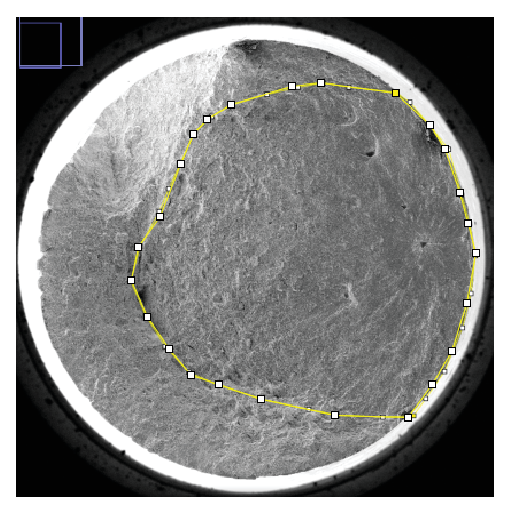
\includegraphics[width=3in]{P1MF19.eps}
  \caption{The crack in model P1MF19 marked with a yellow polygon.}
  \label{fig:P1MF19}
   \end{center}
\end{figure*}
%
The crack was marked manually.
The crack area is 11.118~mm$^2$ and the size of the ligament is $A_{\mbox{uncracked area}}=8.12$~mm$^2$.
Using eq.~(\ref{eq:sig_net}) and noting $\sigma_0=634$~MPa,
                           $\sigma_{net}=1502$~MPa.
The value found is much higher than the allowed stress $\sigma_f=1092$~MPa [how to cite Carmel confidential work??].
This finding shows the need for automatic marking of the crack.


%
%
Here continued the detail on the $\sigma_{net}$ AI model.

%%%%%%%%%%%%%%%%%%%%%%%%%%%%%%%%%%%%%%%%%%%%%%%%

Next, an example of a calculation of $K$ is presented.
The calculation is conducted for specimen P1MF19.
In order to use equation~(\ref{eq:K_I__F_I}), the crack front is approximated as an ellipse, as shown in Fig.~\ref{fig:P1MF19_elip_crack}.
%
\begin{figure*}[t!]
  \begin{center}
  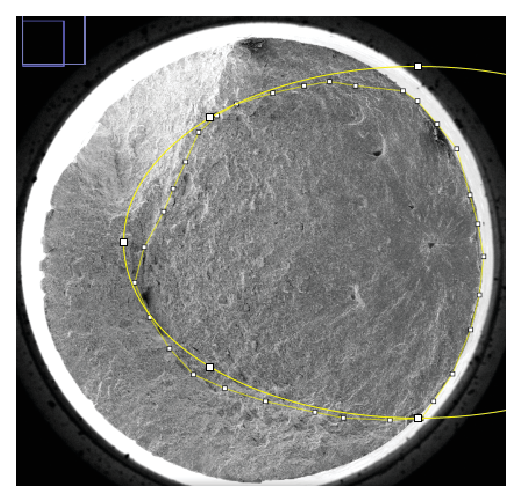
\includegraphics[width=3in]{P1MF19_elip_crack.eps}
  \caption{The crack in model P1MF19 marked with a yellow ellipse.}
  \label{fig:P1MF19_elip_crack}
   \end{center}
\end{figure*}
%
The ellipse was marked manually.
The values of $a, b$ and $D$ are 4.5~mm, 4~mm and 4.9~mm, respectively.
The range of the value $a/b$ in~\cite{shin2004experimental} is between 0 to 1.
Since here $a$ is larger than $b$, the aspect ratio between them is taken as 1.
The value of $F_I$ for $\frac{a}{b}=0, \frac{a}{D}=0.454$ and $\frac{x}{h}=0$, using eq.~(\ref{eq:F_I}), is ~1.042 (Need to be checked with the real equation. I took it from the table in~\cite{shin2004experimental}).
This is the value of $F_I$ at the middle of the crack front.
The value of $F_I$ for $\frac{a}{b}=0, \frac{a}{D}=0.454$ and $\frac{x}{h}=1$, using eq.~(\ref{eq:F_I}), is ~1.402 (kana"l).
This is the value of $F_I$ at the edges of the crack front.
Using eq.~(\ref{eq:K_I__F_I}) and noting $\sigma_0=634$~MPa, $K_I=56~\mbox{MPa}\sqrt{\mbox{m}}$ and $K_I=75\mbox{MPa}\sqrt{\mbox{m}}$ at the middle and at the edges of the crack front, respectively.
The value of the critical stress intensity factor, $K_Ic$, is $70~\mbox{MPa}\sqrt{\mbox{m}}$.
The value of $K_I$ at the middle of the crack front is much lower than the critical value.
The value of $K_I$ at the edges of the crack front is similar to the critical value.
It seems that the reason of the failure is due to the large $\sigma_{net}$ presented in Section~\ref{Subsec: Flow stress calculation model}.
The large value of $K_{Ic}$ at the edges of the crack front is unreasonable.
If the value was indeed such large, the crack should have propagated to the edges and not at the middle of the crack front.



\section{Conclusions and future work}
\label{Sec: Conclusions and future work}
\textcolor{green}{summary\\advantages of the heat map and the automatic calculation}

\section{Acknowledgments}
This work was supported by the ..


%% The Appendices part is started with the command \appendix;
%% appendix sections are then done as normal sections
%% \appendix




%\begin{thebibliography}{00}


 \bibliographystyle{elsarticle-num}
 \bibliography{bibs}




%\end{thebibliography}
\end{document}
\endinput
%%
%% End of file `elsarticle-template-num.tex'.
